In recent years wide cloud adoption has caused huge momentum in adopting software architecture known as micro-services, as it is a native architecture for the cloud. This project will also adapt this architecture because part of the deployment is being done in the cloud, and a swarm of agents can also be simulated using this approach. Moreover, technologies such as kind and tilt made it easier to develop all services locally using the local Kubernetes cluster.

Micro-services are small autonomous services that cooperate with each other to create certain application logic\cite{building_microservices}. Usually, microservices are deployed as Linux containers and encapsulate logic for a single logical part of the solution. Those services are then communicating whit each other to build bigger, more complex systems.

\begin{figure}[H]
    \centering
    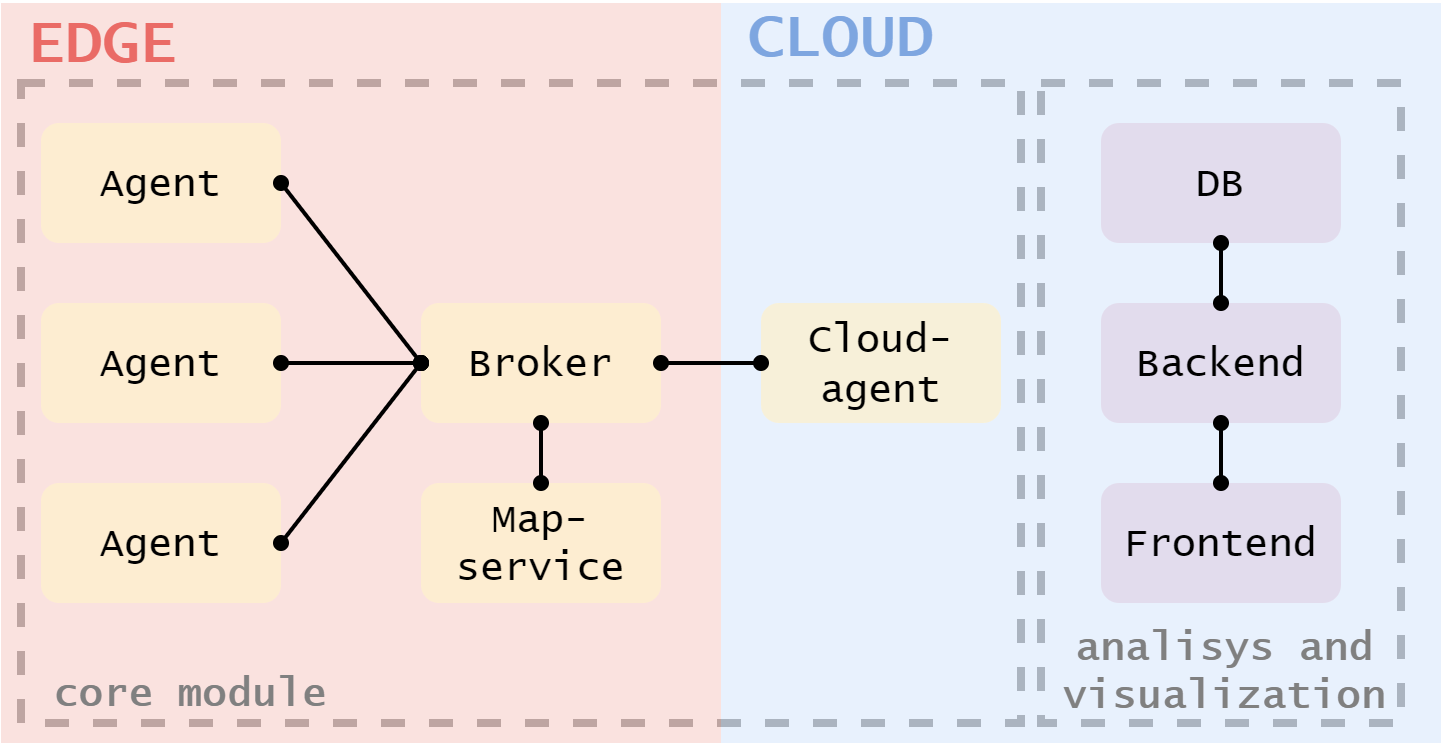
\includegraphics[width=\textwidth]{pictures/services.png}
    \caption{ Microservices system design }
    \label{fig:micro_services}
\end{figure}

\subsection{Agent}
The agent is a microservice which is implementing the logic of the entity which needs to plan a path.  It is meant to have limited resources to simulate a real-world scenario, and the number of its instances will vary.

When an agent is started, it doesn't belong to any swarm so it will start local discovery to find its peers. After peers are found, one of the agents has to be elected as a leader and therefore election algorithm will be initiated in one or multiple agents, so one of the agents will be elected to be a swarm leader. An agent will periodically poll his peers to check their liveness and this behavior will be referred to as a liveness check.

This entity contains also all algorithms meant for path planning as in a base case scenario, computation will take place in the agent to obtain the path.

\subsection{Cloud-agent}
Cloud-agent is an entity to which computation can be upstream to offload the agents. It will have much more computing power, but it might be located in a different geographical location so latency between local agents and this one will matter in the case of total calculation time.

This microservice will be deployed in the cloud and it will use cloud-broker as a communication medium.

\subsection{Broker}
Service is responsible for communication between the services. It will be deployed both in the cloud and in the local environment, and those two entities should be connected with a bridge. This will be a single connection point between the cloud and the edge. This entity will use pub/sub approach to handle and distribute the messages.

\subsection{Map-service}
Initially, when agents are spawned they do not have any map assigned. After electing a leader he will trigger new map generation, by message passing to map-service. This entity is responsible for creation the map and spawning the agent in it. It is a substitute for sensing for the agent as it gives the robots all information they need for finding in position on a global map.

Additionally, pre-defined maps are stored in this service and can be adopted by the agent upon a specific query. Map service can spawn agents in places from which it is not possible to reach the goal, but it is also a valid scenario.

\subsection{Backend}
It is a service meant for gathering data and interacting with a core module(agent, map service, etc.). It exposes the endpoint through REST API (endpoints in appendix A) and forwards requests to the MQTT broker. It is also receiving data from all the entities and stores it in a database connected to it. The backend is deployed in a cloud and it connects to a cloud broker, endpoints should be exposed to the end-user.

\subsection{Frontend}
The end user graphical interface, deployed as a web service is called frontend. It is taking inputs from the user and triggers specific actions through the backend service API. It is also used for raw data visualization and it is deployed in a cloud and exposed to end users. Its capabilities are explained in \hyperref[sec:0308]{visualization section} of this chapter.